\documentclass[letterpaper,final,12pt,reqno]{amsart}

\usepackage[total={6.3in,9.2in},top=1.1in,left=1.1in]{geometry}

\usepackage{empheq}
\usepackage[dvipsnames]{xcolor}
\usepackage{graphicx}
\usepackage{fancyvrb}

%\usepackage{palatino}

% hyperref should be the last package we load
\usepackage[pdftex,
colorlinks=true,
plainpages=false, % only if colorlinks=true
linkcolor=blue,   % only if colorlinks=true
citecolor=Red,   % only if colorlinks=true
urlcolor=black     % only if colorlinks=true
]{hyperref}

\renewcommand{\baselinestretch}{1.05}

\newcommand{\ddt}[1]{\ensuremath{\frac{\partial #1}{\partial t}}}
\newcommand{\ddx}[1]{\ensuremath{\frac{\partial #1}{\partial x}}}
\newcommand{\ddy}[1]{\ensuremath{\frac{\partial #1}{\partial y}}}
\newcommand{\pp}[2]{\ensuremath{\frac{\partial #1}{\partial #2}}}
\renewcommand{\t}[1]{\texttt{#1}}
\newcommand{\Matlab}{\textsc{Matlab}\xspace}
\newcommand{\eps}{\epsilon}
\newcommand{\RR}{\mathbb{R}}

\newcommand{\grad}{\nabla}
\newcommand{\Div}{\nabla\cdot}
\newcommand{\trace}{\operatorname{tr}}


\newcommand{\hbn}{\hat{\mathbf{n}}}

\newcommand{\bg}{\mathbf{g}}
\newcommand{\bu}{\mathbf{u}}
\newcommand{\bv}{\mathbf{v}}

\newcommand{\bX}{\mathbf{X}}



\begin{document}
\graphicspath{{figures/}}

\title[Appendix A: A finite element Stokes solver for glacier flow]{Appendix A: A finite element Stokes solver \\ for glacier flow}

\author{Ed Bueler}

\maketitle

\vspace{-8mm}
\begin{center}
\footnotesize
\emph{\today}
\end{center}

\bigskip

\renewcommand{\theequation}{A\arabic{equation}}

This document is an appendix to my notes \emph{Numerical modelling of glaciers, ice sheets, and ice shelves}---here called ``the notes''---which are used for the International Summer School in Glaciology in McCarthy, Alaska.

We start by stating the Stokes model with glacier-suitable boundary conditions.  Next we construct slab-on-a-slope solutions both for verification and to clarify the boundary conditions.  Then we derive the ``weak form,'' as explained below.  An overview of finite element (FE) methods \cite{Elmanetal2014}, which are based on such weak forms, follows.  Our particular FE method uses triangular elements for an arbitrary planar region and stable mixed elements; these ideas will be only briefly explained.

The main goal of this appendix comes next, namely to generate a numerical solution to a 2D glacier flow with a step in the bedrock (Figure \ref{fig:stepflowlin}).  This numerical solution uses four advanced open source tools/libraries:
\begin{itemize}
\item Gmsh, a mesh generator \hfill \url{http://gmsh.info/}
\item Firedrake, an FE library \hfill \url{https://www.firedrakeproject.org/}
\item PETSc, a solver library \hfill \url{http://www.mcs.anl.gov/petsc/}
\item Paraview, a visualization tool \hfill \url{https://www.paraview.org/}
\end{itemize}
These tools are driven by two short Python codes which are included at the end.

\begin{figure}[h]
\label{fig:stepflowlin}
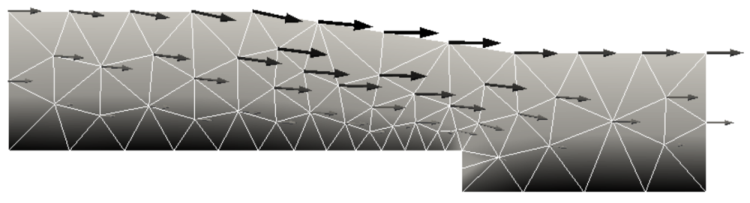
\includegraphics[width=0.8\textwidth,angle=-5.7296]{stepflowlin}  % 0.1 radian = 5.7296 degrees
\caption{A glacier flowing over a bedrock step.  Arrows show velocity $\bu$.  Shading is pressure $p$.  Note the coarse mesh of triangular finite elements.}
\end{figure}


\section{Stokes equations}

Recall the Glen-Stokes model in equations (3), (4), (5) from the notes.  (It is also stated in \cite{GreveBlatter2009,JouvetRappaz2011}.)  The model applies on a 3D or 2D domain $\Omega$ according to the context.  Allowing any Glen exponent $n\ge 1$, the equations are:
\begin{align}
\nabla \cdot \bu &= 0 &&\text{\emph{incompressibility}} \label{incompressible} \\
- \nabla \cdot \tau + \nabla p &= \rho \bg &&\text{\emph{stress balance}} \label{forcebalance} \\
D\bu &= A_n |\tau|^{n-1} \tau &&\text{\emph{Glen flow law}} \label{flowlaw}
\end{align}
The velocity $\bu$, pressure $p$, ice density $\rho$, acceleration of gravity $\bg$, deviatoric stress tensor $\tau$ and strain rate tensor $D\bu$ all appear.  Recall $D\bu$ involves derivatives of velocity:
\begin{equation}
(D\bu)_{ij} = \frac{1}{2} \left((u_i)_{x_j} + (u_j)_{x_i}\right) \label{strainrate}
\end{equation}

Though the notation here generally follows Table 1 in the notes, some usage is more general or flexible.  For example, $A_n$ in \eqref{flowlaw} is the $n$-dependent ice softness.  Table 1 shows $A = A_3 = 10^{-16} \,\text{Pa}^{-3}\,\text{a}^{-1} = 3.1689 \times 10^{-24} \,\text{Pa}^{-3}\,\text{s}^{-1}$, but generally the units of $A_n$ are $\text{Pa}^{-n}\,\text{s}^{-1}$.  Regarding tensor norm notation we have:
\begin{align*}
|\tau|^2 = \frac{1}{2} \trace\left(\tau^2\right) = \frac{1}{2} \tau_{ij} \tau_{ij}, \qquad |D\bu|^2 = \frac{1}{2} \trace\left((D\bu)^2\right) = \frac{1}{2} (D\bu)_{ij} (D\bu)_{ij}
\end{align*}
In the last two expressions the Einstein summation is used over indices $i,j=1,2,3$ or $i,j=1,2$ according to dimension.

Tensors $D\bu$ and $\tau$ are symmetric and have trace zero.  The full (Cauchy) stress tensor $\sigma$ is the deviatoric stress tensor $\tau$ minus the pressure,
\begin{equation}
    \sigma = \tau - p\,I,  \label{cauchystress}
\end{equation}
so equation \eqref{forcebalance} is simply $-\Div \sigma = \rho \bg$.  One may derive that $p = -\frac{1}{3} \trace(\sigma)$ thus that the pressure is the negative of the average normal stress.  By definition $\Div\tau$ in \eqref{forcebalance} is a vector with components which we take to be the divergences of the rows:
    $$\left(\nabla \cdot \tau\right)_i = \left(\tau_{i1}\right)_{x_1} + \left(\tau_{i2}\right)_{x_2} + \left(\tau_{i3}\right)_{x_3}$$
Thus $\nabla\cdot \tau$ is a column vector like $\nabla p$ and $\bg$ in \eqref{forcebalance}.

Recall the viscosity form of flow law \eqref{flowlaw}, namely equation (15) in the notes:
\begin{equation}
\tau = 2\nu D\bu = B_n |D\bu|^{\frac{1}{n} - 1} D\bu  \label{viscflowlaw}
\end{equation}
Here $B_n = (A_n)^{-1/n}$ is the $n$-dependent ice hardness.  With this expression we can eliminate $\tau$ and rewrite equations \eqref{incompressible}, \eqref{forcebalance} in terms of velocity and pressure as
\begin{align}
\Div \bu &= 0 \label{incompagain} \\
- \nabla \cdot \left(B_n |D\bu|^{\frac{1}{n} - 1} D\bu\right) + \nabla p &= \rho \mathbf{g} \label{stokes}
\end{align}
The Stokes model is, from now on, equations \eqref{incompagain}, \eqref{stokes} with certain boundary conditions.  The solution is the velocity-pressure pair $(\bu,p)$.

The domain $\Omega$ must have a smooth-enough boundary to apply the boundary conditions but it is otherwise general.  However, certain glacier-suitable boundary conditions are used in this document and in the code below.  To explain these, consider the numerical solution shown in Figure \ref{fig:stepflowlin}.  We assume that base, top, inflow, and outflow boundary surfaces are all well-defined.  On the base we require no slip:
\begin{align}
\bu &= 0  &&\text{\emph{base}} \label{basebc} \\
\intertext{On the top we set a condition of zero normal stress, $\sigma\hbn=0$ or equivalently:}
\left(B_n |D\bu|^{\frac{1}{n} - 1} D\bu - pI\right) \hbn &= 0  &&\text{\emph{top}} \label{topbc} \\
\intertext{As shown in Figure \ref{fig:stepflowlin}, the left-side inflow boundary is a surface with outward normal $\hbn=\left<-1,0,0\right>^\top$ in all cases we solve.  On this surface we set a nonzero inflow velocity:}
\bu &= \left<f(z),0,0\right>^\top  &&\text{\emph{inflow}} \label{inflowbc} \\
\intertext{(Velocity $f(z)$ will satisfy the slab-on-slope equations; see below.)  On the outflow boundary, where $\hbn=\left<1,0,0\right>^\top$ is the outward normal, $h$ is the surface elevation, and $g=|\bg|$, we set a nonzero hydrostatic normal stress:}
\left(B_n |D\bu|^{\frac{1}{n} - 1} D\bu - pI\right) \hbn &= \left<-\rho g (h-z),0,0\right>^\top  &&\text{\emph{outflow}} \label{outflowbc}
\end{align}


\section{Slab-on-slope solutions}

Testing a numerical model requires verification tools, namely exact solutions.  Thus we recapitulate the construction of the slab-on-slope solutions which was given in the notes, but this time allowing any Glen exponent $n$.  We determine the $n$-dependent ice hardness $B_n$ so that these solutions have the same surface velocity for any $n$.

Suppose the domain $\Omega$ is 2D, the points $(x,y,z)$ where $y=0$.  Denote the components of velocity as $\bu=\left<u,v,w\right>$.  Suppose there is no variation in the cross-flow direction ($\partial/\partial y=0$) and no cross-flow velocity ($v=0$).  Also assume the force of gravity is downward but at angle $\alpha$ with the $z$-direction so $\bg = \left<g\sin\alpha,0,-g\cos\alpha\right>$ where $g=|\bg|$.  Equations \eqref{incompagain}, \eqref{stokes} now become the system
\begin{align}
u_x + w_z &= 0 \label{planeincomp} \\
- \left(B_n |D\bu|^{\frac{1}{n}-1} u_x\right)_x - \left(B_n |D\bu|^{\frac{1}{n}-1} \frac{1}{2} \left(u_z+w_x\right)\right)_z + p_x &= \rho g\sin\alpha \label{planestressx} \\
- \left(B_n |D\bu|^{\frac{1}{n}-1} \frac{1}{2} \left(u_z+w_x\right)\right)_x - \left(B_n |D\bu|^{\frac{1}{n}-1} w_z\right)_z + p_z &= -\rho g\cos\alpha \label{planestressz}
\end{align}
The strain-rate norm expands/simplifies to
\begin{equation}
    |D\bu| = \sqrt{\frac{1}{2} \left(u_x^2 + \frac{1}{2}(u_z+w_x)^2 + w_z^2\right)}  \label{planeDnorm}
\end{equation}
These equations are the 2D (strong) form of the Stokes model, as written-out using coordinates $(x,z)$ and velocity $\bu=\left<u,w\right>$.

Now suppose there is no variation in $x$, i.e.~that $\partial/\partial_x=0$, and that the domain $\Omega$ is a slab such that $b < z < h$ for fixed ($x$-independent) values of the bed elevation $b$ and the surface elevation $h$.  This is the situation of an infinitely-long (or periodic) slab flow with $x$-independent boundary stresses (e.g.~no lubricated spots at the base).  Then the system simplifies to $w_z=0$ and the simplified stress equations
\begin{equation}
- \left(B_n |D\bu|^{\frac{1}{n}-1} \frac{1}{2} u_z\right)_z = \rho g\sin\alpha, \quad
- \left(B_n |D\bu|^{\frac{1}{n}-1} w_z\right)_z + p_z = -\rho g\cos\alpha \label{slabstresses}
\end{equation}
The strain-rate norm simplifies to $|D\bu| = \sqrt{\frac{1}{2} \left(\frac{1}{2}u_z^2 + w_z^2\right)}$.

If we further assume that there is no slip at the base then $w=0$ identically.  Then the second of equations \eqref{slabstresses} allows integration with respect to $z$.  Assuming zero pressure at the surface gives $p = \rho g\cos\alpha (h-z)$.  Also $|D\bu| = \frac{1}{2} |u_z|$.  From \eqref{slabstresses} we now have a single nontrivial equation to solve for the horizontal velocity:
    $$- \left(\frac{B_n}{2^{\gamma+1}} |u_z|^\gamma u_z\right)_z = \rho g\sin\alpha$$
The flow of a viscous, non-sliding fluid on a uniform slab will be such that $u_z>0$.  With rearrangement, the equation is now
    $$\left((u_z)^{1/n} \right)_z = - \frac{2^{1/n} \rho g\sin\alpha}{B_n}$$
Again this can be integrated from the surface $z=h$, using the no-stress (no traction) condition, which becomes $u_z=0$, to give
    $$u_z = 2 \left(\frac{\rho g\sin\alpha}{B_n}\right)^n (h-z)^n.$$
Integrating vertically one more time, from the base $z=b$ where $u=0$, gives
\begin{equation}
u(z) = \frac{2}{n+1} \left(\frac{\rho g\sin\alpha}{B_n}\right)^n \left((h-b)^{n+1} - (h-z)^{n+1}\right)  \label{uslab}
\end{equation}

Suppose our goal is to generate comparable solutions with glaciologically-reasonable ice velocities for any $n\ge 1$.  Ice sheet modeling tradition \cite{GreveBlatter2009}, and glaciological experiments starting with Glen, suggest we base our work on $n=3$.  From the ice softness value $A_3 = 3.1689 \times 10^{-24} \,\text{Pa}^{-3}\,\text{s}^{-1}$ we get $B_3 = (A_3)^{-1/3} = 6.8082\times 10^7\,\text{Pa}\,\text{s}^{1/3}$.  We now compute $B_n$ for any $n\ge 1$ so the slab-on-slope surface velocity $u(h)$ from \eqref{uslab} matches the value in the $n=3$ case.  Thus we determine $B_n$ from the equation
    $$\frac{2}{n+1} \left(\frac{\rho g\sin\alpha}{B_n}\right)^n (h-b)^{n+1} = \frac{1}{2} \left(\frac{\rho g\sin\alpha}{B_3}\right)^3 (h-b)^4$$
which reduces to
\begin{equation}
B_n = \left(\frac{4}{n+1}\right)^{1/n} \Big(\rho g \sin\alpha (h-b)\Big)^{(n-3)/n} {B_3\,}^{3/n}  \label{Bnfromsurface}
\end{equation}
For example, suppose $h-b=400$ m and $\alpha=0.1$ radian (about $5.7$ degrees).  When we use $B_n$ from \eqref{Bnfromsurface} we get a surface velocity of $u(h)=906.09 \,\text{m}\,\text{a}^{-1}$ from \eqref{uslab} for any $n\ge 1$.  The result from \eqref{Bnfromsurface} itself is $B_1=4.9663\times 10^{12}\,\text{Pa}\,\text{s}$ and $B_4=1.7320\times 10^{7}\,\text{Pa}\,\text{s}^{1/4}$, to mention some glaciologically-relevant end-cases $n=1,4$ \cite{GreveBlatter2009}.  The Newtonian viscosity $\nu=B_1/2$ is about $10^{16}$ times more viscous than liquid water but about $10^7$ times less viscous than granite (both at $25^\circ \,\text{C}$).


FIXME compute normal stress on outflow face


\section{Weak form}

The Stokes equations \eqref{incompagain}, \eqref{stokes} are PDEs called the \emph{strong form} of the model.  The \emph{weak form}, needed to construct an FE method, is derived by multiplying the equations by arbitrary test functions and then integrating over $\Omega$ so as to define a scalar-valued nonlinear functional $F$.  In the FE method the test functions will be locally constructed from the triangular mesh.

The solution is the pair $(\bu,p)$ where $\bu\in V_D$ and $p \in Q$ for function spaces precisely identified in \cite{JouvetRappaz2011}.  The test functions come from nearly the same spaces but with differences relating (only) to the value of Dirichlet boundary conditions: the solution velocity $\bu\in V_D$ satisfies \eqref{basebc}, \eqref{inflowbc} while the test functions $\bv\in V_0$ are zero on both base and inflow surfaces.  The test pressures are from $Q$ just like $p$.

We multiply \eqref{incompagain} by $q\in Q$ and \eqref{stokes} by $\bv\in V_0$, and combine to define $F$:
\begin{equation}
F(\bu,p;\bv,q) = \int_\Omega - \left(\nabla \cdot \left(B_n |D\bu|^{\frac{1}{n} - 1} D\bu\right)\right)\cdot \bv + \nabla p \cdot \bv - \rho \mathbf{g} \cdot \bv - \left(\nabla \cdot \bu\right) q \label{nonfuncone}
\end{equation}
The nonlinear functional must be zero at the solution $(\bu,p)$ in the sense that $F(\bu,p;\bv,q) = 0$ for all  $\bv\in V_0$ and $q\in Q$.

Integration-by-parts rewrites $F$ to balance the derivatives on $(\bv,q)$ and $(\bu,p)$.  Recall the product rule $\nabla \cdot(f\bX) = \grad f\cdot \bX + f \nabla \cdot \bX$ and the divergence theorem $\int_\Omega \nabla \cdot \bX = \int_{\partial \Omega} \bX \cdot \hbn$.  Again denoting $\tau = B_n |D\bu|^{\frac{1}{n} - 1} D\bu$ we have
\begin{align*}
\int_\Omega \left(\nabla \cdot \tau\right)\cdot \bv &= \sum_{j=1}^3 \int_\Omega \nabla \cdot (\tau_{j\circ})\, v_j = \sum_{j=1}^3 \int_\Omega \nabla \cdot (\tau_{j\circ}^\top v_j) - \tau_{j\circ}^\top \nabla v_j \\
  &= \sum_{j=1}^3 \int_{\partial \Omega} (\tau_{j\circ}^\top v_j) \cdot \hbn - \int_\Omega \tau_{j\circ}^\top \cdot \nabla v_j = \int_{\partial \Omega} (\tau \hbn)\cdot \bv - \int_\Omega \trace(\tau \nabla \bv)
\end{align*}
where $\circ$ denotes an index iterated-over, $\tau_{j\circ}$ denotes the $j$th row of $\tau$, and $\tau_{j\circ}^\top$ denotes the same vector regarded as a column vector.  Also recall $\grad\bv$ defines a $3\times 3$ matrix,
\newcommand{\trefthree}[3]{\left[\begin{array}{c|c|c} & & \\ #1 & #2 & #3 \\ & & \end{array}\right]}
    $$\grad \bv = \trefthree{\grad v_1}{\grad v_2}{\grad v_3} = \begin{bmatrix}
    (v_1)_{x_1} & (v_2)_{x_1} & (v_3)_{x_1} \\
    (v_1)_{x_2} & (v_2)_{x_2} & (v_3)_{x_2} \\
    (v_1)_{x_3} & (v_2)_{x_3} & (v_3)_{x_3}
    \end{bmatrix}$$
so
    $$\trace(\tau \grad \bv) = \sum_{j=1}^3 \tau_{j\circ}^\top \cdot \grad v_j = \sum_{i,j=1}^3 \tau_{ji} (v_j)_{x_i}$$
Also, because $\trace(AB)=0$ if $A$ is symmetric and $B$ is antisymmetric, in fact $\trace(\tau \grad \bv) = \trace(\tau D\bv)$.  (To show this take $A=\tau$ and $B=\grad\bv-D\bv$.)  Regarding notation in other sources, for the Stokes equations it is common to write $A:B$ for $\trace(AB)$.

In addition we do a straightforward integration-by-parts on the pressure portion:
    $$\int_\Omega \nabla p \cdot \bv = \int_\Omega \nabla\cdot (p\,\bv) - p (\nabla \cdot \bv) = \int_{\partial \Omega} p\hbn \cdot \bv - \int_\Omega p (\nabla \cdot \bv)$$
These facts, plus denoting $\sigma=\tau-pI$ for clarity, allow us to rewrite \eqref{nonfuncone} with an integral of the normal stress over the boundary:
\begin{equation}
F(\bu,p;\bv,q) = -\int_{\partial\Omega} (\sigma \hbn)\cdot \bv + \int_\Omega \trace(\tau D\bv) - p (\nabla \cdot \bv) - \left(\nabla \cdot \bu\right) q - \rho \mathbf{g} \cdot \bv \label{nonfunctwo}
\end{equation}
Note that $\bu,\bv$ now appear with at most first derivatives and $p,q$ appear only without derivatives in \eqref{nonfunctwo}.

Recall that $\bv\in V_0$ satisfies $\bv=0$ along the base and inflow surfaces so these portions of the above integral over $\partial\Omega$ are zero.  Conditions \eqref{topbc}, \eqref{outflowbc} therefore completely eliminate the unknown solution $\bu,p$ from the boundary integral, and this yields our final formula for the nonlinear functional:
\begin{align}
F(\bu,p;\bv,q) &= \int_\Omega B_n |D\bu|^{\frac{1}{n} - 1} \trace(D\bu D\bv) - p (\nabla \cdot \bv) - \left(\nabla \cdot \bu\right) q \label{defineF} \\
    &\qquad  - \int_\Omega \rho \mathbf{g} \cdot \bv - \int_{\{\text{outflow}\}} \rho g (h-z) v_1  \notag
\end{align}
The last two integrals can be regarded as the source terms.  For example, if we replace them by zero---no gravity or outflow stress---then we expect solution $\bu=0$ and $p=0$.

The weak formulation of the Stokes model is the statement that $F$ is zero in all directions at the solution: the solution $\bu\in V_D$ and $p\in Q$ satisfies
\begin{equation}
F(\bu,p;\bv,q) = 0 \qquad \text{ for all } \bv\in V_0 \text{ and } q\in Q  \label{weak}
\end{equation}
This weak formulation is proven in \cite{JouvetRappaz2011} to be well-posed under reasonable assumptions about the domain $\Omega$ and boundary data which will be satisfied in the cases we consider.  Thus there is exactly one solution pair $(\bu,p)$.  From now on our goal is to approximate this solution numerically.


\section{Finite element method}

FIXME

\section{Firedrake code}

FIXME: show block figure with blocks = (genstepmesh.py,gmsh,flowstep.py,paraview) and file formats as arrows (.geo,.msh,.pvd)

FIXME: show codes here

%\VerbatimInput[frame=lines,numbers=left,stepnumber=5,fontsize=\footnotesize]{../genstepmesh.py}

%\VerbatimInput[frame=lines,numbers=left,stepnumber=5,fontsize=\footnotesize]{../flowstep.py}

\footnotesize

\bigskip
%from: \bibliographystyle{siam}

\begin{thebibliography}{6}

\bibitem{BaliseRaymond1985}
{\sc M.~Balise and C.~Raymond}, {\em Transfer of basal sliding variations to
  the surface of a linearly-viscous glacier}, J. Glaciol., 31 (1985),
  pp.~308--318.

\bibitem{Brownetal2013}
{\sc J.~Brown, B.~Smith, and A.~Ahmadia}, {\em Achieving textbook multigrid
  efficiency for hydrostatic ice sheet flow}, SIAM J. Sci. Computing,
  35 (2013), pp.~B359--B375.

\bibitem{Elmanetal2014}
{\sc H.~C. Elman and D.~J. Silvester and A.~J. Wathen}, {\em Finite Elements
  and Fast Iterative Solvers: with Applications in Incompressible Fluid Dynamics},
  Oxford University Press, 2nd~ed., 2014.

\bibitem{GreveBlatter2009}
{\sc R.~Greve and H.~Blatter}, {\em Dynamics of {I}ce {S}heets and {G}laciers},
  Advances in Geophysical and Environmental Mechanics and Mathematics,
  Springer, 2009.

\bibitem{JouvetRappaz2011}
{\sc G.~Jouvet and J.~Rappaz}, {\em Analysis and finite element approximation
  of a nonlinear stationary {S}tokes problem arising in glaciology}, Advances
  in Numerical Analysis, (2011).

\bibitem{Lengetal2012}
{\sc W.~Leng, L.~Ju, M.~Gunzburger, S.~Price, and T.~Ringler}, {\em A parallel
  high-order accurate finite element nonlinear {S}tokes ice sheet model and
  benchmark experiments}, J. Geophys. Res., 117 (2012).

\end{thebibliography}


\end{document}
